\chapter{Referencial Teórico}

O desenvolvimento do AgroSíntese está fundamentado em um conjunto de referenciais teóricos que abordam a linguagem, a comunicação, a experiência e a extensão rural sob uma perspectiva crítica, dialógica e situada. A proposta da plataforma ultrapassa a ideia de simples automatização do atendimento técnico e se constitui como uma prática comunicativa que valoriza os saberes locais, a escuta ativa e o reconhecimento dos sujeitos do campo como protagonistas da construção do conhecimento. A seguir, discutimos os principais aportes teóricos que sustentam a concepção deste sistema.

\section{A linguagem como fenômeno dialógico e social}

A obra de Mikhail Bakhtin constitui uma das principais bases teóricas para o AgroSíntese. Em "Estética da Criação Verbal" \cite{bakhtin1997estetica}, o autor propõe uma concepção de linguagem que é essencialmente dialógica, marcada por relações sociais e históricas que se manifestam nos enunciados. Para Bakhtin, toda fala se dá em resposta a outra fala, e todo enunciado está inserido em uma cadeia viva de interlocuções. Essa perspectiva dialogada fundamenta a proposta de um sistema que não apenas responde a comandos ou perguntas, mas interage, reconhece os sentidos contextuais e se adapta linguisticamente ao universo do interlocutor.

Essa ideia é aprofundada em "Marxismo e Filosofia da Linguagem" \cite{bakhtin1981marxismo}, onde o autor (sob o pseudônimo de Volochínov) critica a linguística formalista e propõe uma abordagem sociológica da linguagem. Aqui, o sentido das palavras não é fixo, mas resultado das condições sociais em que são produzidas e apropriadas. Assim, para que o AgroSíntese seja eficaz, é fundamental que ele reconheça e incorpore os regionalismos, gírias e variações linguísticas dos territórios rurais brasileiros como partes legítimas do processo comunicativo.

\section{Educação dialógica e comunicação libertadora}

Paulo Freire \cite{freire2013extensao}, em sua obra "Extensão ou Comunicação?", questiona o modelo de extensão rural tradicional, que trata o agricultor como um sujeito passivo a ser instruído. Para Freire, essa lógica é marcada por uma visão bancária da educação, em que o conhecimento é depositado no outro. Em oposição, ele propõe uma educação dialógica, baseada na troca, na escuta, no respeito ao saber popular e na construção conjunta do conhecimento. Essa concepção está presente no AgroSíntese, que se estrutura não como um sistema de respostas prontas, mas como uma ferramenta que estimula o diálogo e reconhece o agricultor como sujeito do processo de aprendizagem.

A crítica freiriana à "extensão" como imposição se materializa no esforço do AgroSíntese de incorporar elementos da cultura local, sotaques regionais e vocabulários populares, oferecendo um atendimento que respeita a identidade linguística e cultural dos usuários. A IA utilizada na plataforma é treinada não apenas com dados técnicos, mas também com registros e expressões do cotidiano rural, de modo a estabelecer uma comunicação horizontal e significativa.

\section{A experiência como fundamento da significação}

Jorge Larrosa \cite{larrosa2014}, ao refletir sobre a experiência, destaca que ela se dá quando algo nos atravessa e nos transforma. Não é suficiente que a informação chegue até o sujeito; é preciso que ela se torne experiência, que produza sentido, que seja sentida, elaborada, incorporada. No contexto da extensão rural, isso implica reconhecer que o simples repasse de informações técnicas não é suficiente. É preciso que o conhecimento faça sentido na vida do agricultor, que dialogue com sua prática, seu território, seu tempo e sua história.

A proposta do AgroSíntese reconhece esse princípio ao oferecer um atendimento que respeita os ritmos e modos de vida do agricultor. O sistema busca produzir sentido ao adaptar-se ao contexto regional, respeitar os modos de fala, as práticas locais e os saberes tradicionais. A comunicação gerada pela plataforma visa gerar experiências, e não apenas transmissões técnicas.

\section{A comunicação rural e a ATER digital participativa}

Zuin \cite{zuin2021comunicacao} destaca que a comunicação rural deve considerar os fluxos de sentido próprios dos territórios, seus tempos, formas de convivência e mediações culturais. A comunicação é parte constitutiva da vida rural e não pode ser reduzida a técnicas ou manuais. Ela é atravessada por afetos, memórias, relações de confiança e oralidades específicas. Lopes et al. \cite{lopes2022}, por sua vez, defendem a ideia de uma ATER digital participativa, que articula saberes acadêmicos e populares, tecnologias digitais e processos educativos dialógicos.

O AgroSíntese incorpora essas concepções ao estruturar um sistema que é, ao mesmo tempo, tecnológico e pedagógico, informacional e formativo. A plataforma não se limita a transmitir dados, mas busca construir pontes entre saberes, mediar o encontro entre diferentes linguagens e reconhecer o agricultor como sujeito do território e do conhecimento.

Assim, o referencial teórico do AgroSíntese sustenta a criação de um ambiente digital que respeita, escuta, dialoga e se adapta, contribuindo para uma extensão rural mais inclusiva, significativa e transformadora.

\section{Sotaque e identidade na comunicação rural}

O sotaque é uma das manifestações mais perceptíveis da identidade regional e cultural de um sujeito. Na tradição da sociolinguística brasileira, os estudos do Projeto ALiB (Atlas Linguístico do Brasil) identificam sete grandes zonas dialetais com traços linguísticos próprios, presentes tanto no léxico quanto na prosódia.

Essas variações, muitas vezes invisibilizadas em iniciativas técnicas e tecnológicas, tornam-se centrais em contextos de educação e extensão rural. Incorporar essas marcas linguísticas nos sistemas automatizados de atendimento técnico é, portanto, uma estratégia não apenas de eficiência comunicativa, mas também de respeito à dignidade cultural dos agricultores.

O AgroSíntese toma o sotaque como elemento-chave da escuta ativa e da comunicação horizontal, promovendo uma experiência dialógica que reconhece a singularidade linguística de cada território.


\section{Heteroglossia aplicada ao campo}
Para Bakhtin \cite{bakhtin2010poetica}, língua é sempre um “campo de batalha” onde diferentes vozes sociais disputam sentido. O AgroSíntese incorpora esse princípio ao mapear 42 dialetos operacionais: cada DDD passa a funcionar como chave de heteroglossia, ativando um modelo acústico e lexical que materializa a voz social daquele território. Assim, quando um agricultor de DDD 85 ouve a resposta no ritmo entoativo cearense, ele reconhece imediatamente seu lugar na cadeia dialógica. Não se trata de simples localização, mas de descentralização enunciativa: a IA abdica da norma culta monolítica e devolve à interação a pluralidade histórica que compõe o português rural brasileiro.


\chapter{Metodologia}

A construção do AgroSíntese será orientada por uma abordagem metodológica qualitativa, participativa e iterativa, centrada no princípio de que as tecnologias devem emergir das necessidades concretas dos sujeitos e dos territórios aos quais se destinam. Inspirado nas diretrizes de uma ATER Digital Participativa \cite{lopes2022}, o desenvolvimento do sistema buscará integrar o conhecimento técnico-científico com saberes populares, práticas locais e repertórios linguísticos dos agricultores familiares brasileiros.

A metodologia será organizada em quatro eixos interdependentes: (1) mapeamento e escuta dos sujeitos do campo; (2) desenvolvimento da base de conhecimento e dicionários regionais; (3) treinamento e adaptação da inteligência artificial; e (4) testes de usabilidade e retorno dialógico com os usuários. Cada eixo será conduzido com base em práticas dialógicas, inspiradas por \cite{freire2013extensao}  e Bakhtin \cite{bakhtin1997estetica}, priorizando a escuta, a coautoria e a circularidade na produção do sistema.

\section{Mapeamento linguístico e escuta dos territórios}

O processo se iniciará com um mapeamento linguístico-cultural de várias regiões do Brasil, com o objetivo de identificar variações de vocabulário técnico-popular, gírias, expressões idiomáticas e sotaques característicos de cada território. Esse levantamento será realizado por meio de entrevistas abertas com agricultores, extensionistas e educadores populares, além da análise de materiais audiovisuais e documentos locais.

A escuta qualificada será uma etapa central: serão priorizadas narrativas orais que evidenciarão não apenas o modo como se fala, mas também como se organiza o pensamento técnico e cotidiano no campo. Essa etapa será registrada em áudio e transcrita para posterior uso no treinamento da IA, garantindo que os enunciados utilizados no sistema reflitam a linguagem viva dos sujeitos do campo, conforme defendido por Bakhtin \cite{bakhtin1997estetica}.

\section{Criação dos dicionários regionais e ontologias contextuais}

A partir dos dados coletados, serão construídos dicionários de regionalismos e ontologias contextuais para cada território mapeado. Esses dicionários não se restringem a termos técnicos agrícolas, mas incluem expressões populares, estruturas sintáticas recorrentes e elementos de cortesia e afeto típicos de cada região. O objetivo será criar uma camada semântica capaz de mediar a interação entre a linguagem técnica e a linguagem local, permitindo que a IA compreenda e responda de maneira contextualizada e culturalmente sensível.

Cada dicionário será revisado por extensionistas e validado com os próprios agricultores que participarão da coleta, em rodas de conversa orientadas por princípios freirianos. A linguagem do sistema, portanto, será fruto de um processo de escuta, tradução e validação coletiva.

A Tabela~\ref{tab:variacoes-regionais} apresenta como será contruído este dicionário.

\begin{table}[H]
	\centering
	\label{tab:variacoes-regionais}
	\caption{Exemplos de variações regionais de termos rurais}
	\begin{tabular}{|l|l|p{8cm}|}
		\hline
		\textbf{Termo}       & \textbf{Variante regional} & \textbf{Regiões / Dialetos} \\ \hline
		
		Mandioca             & Macaxeira                  & Alagoano (AL), Soteropolitano (BA), Pernambucano (PE), Sergipano (SE), Cearense (CE), Paraibano (PB), Porto-Segurense (BA), Recifense (PE), Paulo-Afonsino (BA) \\ \hline
		
		Mandioca             & Aipim                      & Carioca (RJ), Capixaba (ES), Vitoriense (ES), Paulistano (SP), Brasiliense (DF) \\ \hline
		
		Mandioca             & Mandioca brava             & Gaúcho (RS), Paranaense (PR), Mato-Grossense (MT), Rondoniense (RO), Nortista (AC, PA, AM) \\ \hline
		
		Milho verde          & Espiga                     & Gaúcho (RS), Sulista (PR \& SC), Campineiro (SP), Sorocabano (SP), Catarinense (SC) \\ \hline
		
		Milho cru ralado          & Pamonha  & Cearense (CE), Paraibano (PB), Recifense (PE), Baiano (BA), Sertanejo (PI) \\ \hline
		
		Milho cru ralado          & Caruá     & Manauara (AM), Paraense (PA), Belenense (PA), Rondoniense (RO), Nortista (AC) \\ \hline
		
	\end{tabular}
\end{table}


\section{Adaptação Regional por Sotaques}
\label{subsec:sotaques}

O \textit{Atlas Linguístico do Brasil} (ALiB) delimita sete grandes zonas dialetais
brasileiras, representadas na   ~\ref{fig:mapa-alib}. úteis para uma segmentação inicial de vocabulário, prosódia e construção
sintática \cite{cardoso2014alib}  Entretanto, pesquisas mais recentes --- em
especial a tese de Pagani \cite{pagani2022} --- revelam um mosaico muito mais
fino de variedades, no qual cada capital ou microrregião apresenta traços
fonético-fonológicos e léxicos suficientemente salientes para serem percebidos
pelo falante comum.  
Incorporar essa granularidade é decisivo para aumentar a empatia e a
inteligibilidade do \textit{AgroSíntese}: quando o agricultor escuta o sistema
no seu próprio sotaque, a mensagem deve ser imediatamente reconhecida como “próxima”,
descartando a sensação de distância cultural frequentemente associada a
tecnologias “de fora”.

Com base no mapeamento de Pagani, ampliamos as sete macrorregiões do
ALiB para um total de \textbf{42 dialetos de referência}.
Cada dialeto é vinculado a um único código DDD ― obtido no
\textit{Plano de Numeração de Áreas} da ANATEL \cite{anatel_pnb}, que pode ser visto na  ~\ref{fig:mapa-ddd}.
Tal estratégia responde ao que Bakhtin \cite{bakhtin1981marxismo} denomina ‘palavra com acento local’: o enunciado que carrega consigo as marcas de um grupo social concreto. Ao preservar essas marcas nos módulos TTS/STT, o AgroSíntese cria uma via de mão dupla onde a voz do agricultor não é corrigida, mas acolhida como componente legítimo do processo educativo.
Para isso, o sistema inferirá, a partir do número de telefone, o modelo acústico
e o dicionário lexicográfico corretos para a geração de voz
(\textit{text-to-speech}) e a interpretação da entrada (\textit{speech-to-text}).


\begin{figure}[h]
	\centering
	\caption{Divisão dialetal de Antenor Nascentes em 1922}
	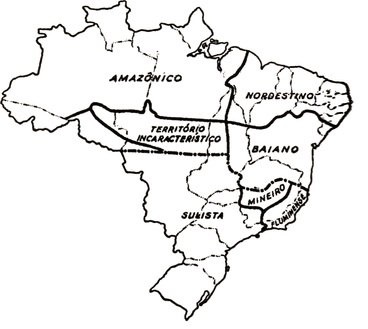
\includegraphics[width=1\linewidth,scale=1.0]{images/mapa-alib.jpg}
	\label{fig:mapa-alib}
\end{figure}


\begin{figure}[h]
	\centering
	\caption{Plano de Numeração adotado no Brasi.  }
	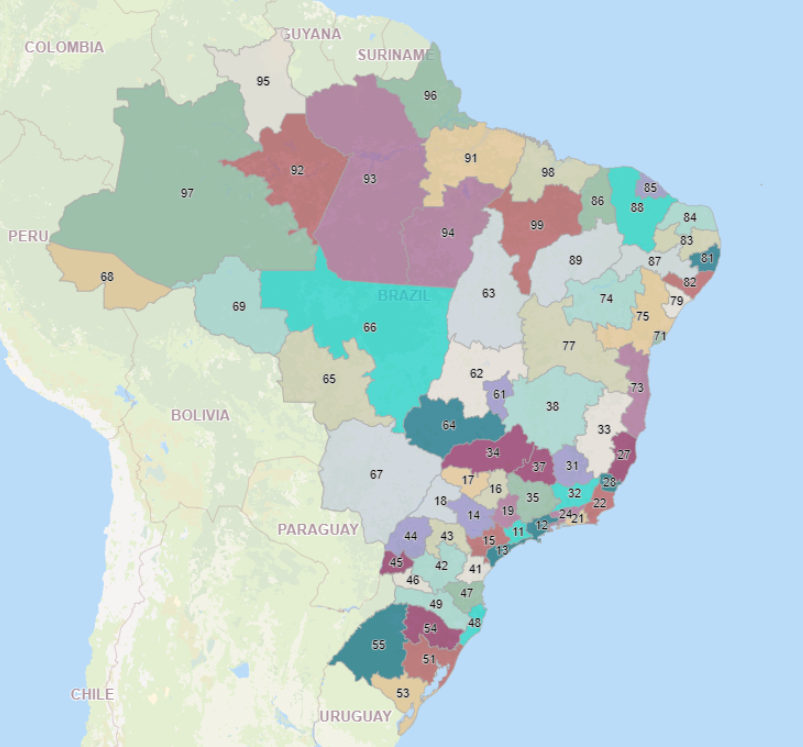
\includegraphics[width=1\linewidth,scale=1.0]{images/mapa-ddd.png}
	\label{fig:mapa-ddd}
\end{figure}


\begin{table}[htbp]
	\centering
	\scriptsize
	\caption{Dialetos brasileiros de referência (Pagani, 2022) e respectivos DDDs exclusivos}
	\label{tab:dialetos_ddd}
	\begin{tabular}{p{3.3cm} p{1.1cm} p{7.7cm} p{0.9cm}}
		\toprule
		\textbf{Dialeto} & \textbf{UF} & \textbf{Localização / caracterização geográfica} & \textbf{DDD}\\
		\midrule
		Alagoano & AL & Todo o estado, do litoral de Maceió à Zona da Mata & 82\\
		Baiano & BA & Interior e litoral baiano em geral & 77\\
		Cearense & CE & Fortaleza e Sertão Central até o Cariri & 85\\
		Maranhense & MA & São Luís e Baixada Maranhense & 98\\
		Nordestino (genérico) & CE, PB, PE, BA, PI & Sertão semiárido do Nordeste & 89\\
		Paraibano & PB & Litoral (João Pessoa) ao agreste/Cariri & 83\\
		Pernambucano & PE & Interior agreste-sertão (exc. Recife) & 87\\
		Porto-Segurense & BA & Município de Porto Seguro & 73\\
		Sergipano & SE & Estado inteiro, núcleo em Aracaju & 79\\
		Soteropolitano & BA & Salvador e Região Metropolitana & 71\\
		Sertanejo & PI, BA, PE & Faixa sertaneja semiárida & 74\\
		Caravelense & BA & Caravelas e litoral sul & --\\
		Recifense & PE & Recife e Região Metropolitana & 81\\
		Paulo-Afonsino & BA & Cidade de Paulo Afonso (norte da BA) & 75\\
		Teresinense & PI & Capital Teresina & 86\\
		Nortista & AC, AP, AM, PA, RO, RR, TO & Interior amazônico & 96\\
		Manauara & AM & Manaus e entorno urbano & 92\\
		Belenense & PA & Belém e Ilha de Marajó & 91\\
		Rondoniense & RO & Porto Velho e interior & 69\\
		Paraense & PA & Interior sudeste + litoral oriental & 93\\
		Carioca & RJ & Cidade do Rio de Janeiro e Baixada Fluminense & 21\\
		Paulista (interior) & SP & Centro-oeste e noroeste paulista & 16\\
		Mineiro & MG & Zona da Mata e Sul de Minas & 35\\
		Capixaba & ES & Estado geral & 28\\
		Vitoriense & ES & Ilha de Vitória e conurbação & 27\\
		Paulistano & SP & Capital e Região Metropolitana de SP & 11\\
		Piracicabano & SP & Piracicaba a Limeira & --\\
		Santista & SP & Baixada Santista & 13\\
		Uberlandense & MG & Uberlândia e Triângulo Mineiro & 34\\
		Sorocabano & SP & Sorocaba e centro-sul paulista & 15\\
		Belo-horizontino & MG & Belo Horizonte e RMBH & 31\\
		Botucatuense & SP & Botucatu e serras centrais & 14\\
		Bragantino & SP & Bragança Paulista / Circuito das Águas & --\\
		Campineiro & SP & Campinas e polo tecnológico & 19\\
		Campo-Belense & MG & Campo Belo (sul de MG) & --\\
		Capão-Bonitense & SP & Capão Bonito e Vale do Paranapanema & --\\
		Paranaense & PR & Interior do estado (exc. Curitiba e litoral) & 43\\
		Gaúcho & RS & Todo o Rio Grande do Sul & 51\\
		Sulista & PR, SC & Planaltos Campos Gerais-Catarinense & 42\\
		Curitibano & PR & Curitiba e Região Metropolitana & 41\\
		Catarinense & SC & Grande Florianópolis + interior & 49\\
		Cascavelense & PR & Cascavel e fronteira oeste & 45\\
		Goiano & GO & Eixo Anápolis-Goiânia-Rio Verde & 62\\
		Mato-Grossense & MT & Cuiabá e centro-sul do estado & 65\\
		Brasiliense & DF & Brasília e cidades-satélite & 61\\
		\bottomrule
	\end{tabular}
\end{table}

A adoção dessa malha dialetal possibilita:

\begin{itemize}
	\item \textbf{Roteamento automático de sotaque}: o DDD do usuário ativa o
	modelo acústico e o dicionário lexical correspondentes;
	\item \textbf{Fine-tuning contextualizado}: as transcrições de áudio coletadas
	em campo realimentam apenas o dialeto pertinente, evitando
	“contaminações” entre variedades;
	\item \textbf{Mensuração de cobertura}: métricas de desempenho são
	estratificadas por dialeto, orientando futuras coletas de voz
	(\emph{speech corpora}) nas regiões com menor acurácia.
\end{itemize}

Dessa forma, o \textit{AgroSíntese} supera a abordagem genérica de “português
brasileiro padrão” e promove uma experiência comunicativa verdadeiramente
situada, alinhada às diretrizes freirianas de diálogo horizontal e ao
reconhecimento bakhtiniano da heterogeneidade constitutiva da linguagem.


\section{Treinamento da Inteligência Artificial}

A IA utilizada no AgroSíntese será baseada na arquitetura GPT4All, customizada e treinada com uma base de dados composta por manuais técnicos, respostas de extensionistas, legislações agrícolas, publicações científicas e, principalmente, transcrições das entrevistas e interações com agricultores. O treinamento envolverá o ajuste fino (fine-tuning) de modelos linguísticos para garantir que as respostas geradas estivessem em consonância com o contexto regional de quem interage com o sistema.

Além da textualização, será incorporado ao sistema um módulo de síntese de voz neural, capaz de reproduzir sotaques regionais com fidelidade, com base nas amostras coletadas e processadas por redes neurais treinadas especificamente para essa finalidade. O objetivo será garantir não apenas compreensão textual, mas também acolhimento e empatia no modo como as mensagens são entregues ao usuário.

\section{Avaliação participativa e iterativa da plataforma}

A última etapa metodológica constituirá na testagem do sistema com grupos de agricultores e técnicos, em contextos reais de uso. Os testes serão conduzidos em ciclos iterativos, com foco na usabilidade, na precisão das respostas, na adequação linguística e na experiência geral de interação. Serão utilizados instrumentos como observação participante, questionários de avaliação e entrevistas pós-uso.

A cada ciclo de testagem, ajustes serão incorporados no banco de dados, na lógica de roteamento de mensagens e na interface do sistema. O retorno dos usuários será documentado e integrado ao processo de desenvolvimento como um elemento central, reafirmando o compromisso com a coautoria e o diálogo, conforme proposto por Freire \cite{freire2013extensao} e pelas práticas de ATER Digital Participativa.

Portanto, a metodologia adotada para o AgroSíntese não apenas orientará tecnicamente o projeto, mas também materializará uma concepção de tecnologia como prática social, comunicativa e educativa, que se contruirá com e para os sujeitos do campo.






\chapter{Desenvolvimento do Sistema}

O presente capítulo descreve a arquitetura técnica e o processo de implementação da plataforma AgroSíntese, detalhando as tecnologias utilizadas, os critérios que orientaram sua escolha, o fluxo de informações entre os diferentes componentes do sistema e os aspectos relacionados à interface com o usuário. Esta etapa representará a concretização dos princípios metodológicos discutidos no capítulo anterior, materializando a proposta de uma ATER digital dialógica, inclusiva e regionalizada.

\section{Tecnologias Utilizadas e Justificativas}

A escolha das tecnologias foi guiada por critérios de acessibilidade, compatibilidade com dispositivos de baixo custo, capacidade de personalização e suporte à integração com sistemas de inteligência artificial e comunicação por voz. A Tabela~\ref{tab:tecnologias} apresenta um resumo das ferramentas e linguagens adotadas.

\begin{table}[H]
	\centering
	\caption{Tecnologias utilizadas na construção do AgroSíntese}
	\label{tab:tecnologias}
	\begin{tabular}{|l|l|l|}
		\hline
		\textbf{Tecnologia} & \textbf{Finalidade} & \textbf{Justificativa} \\
		\hline
		WhatsApp Business API & Canal de interação & Alta adesão no campo brasileiro \\
		Kommo CRM & Integração com WhatsApp & Automação de mensagens \\
		GPT4All & Processamento de linguagem natural & IA treinável localmente\\
		Coqui TTS & Geração de voz sintética & Suporte a sotaques regionais \\
		Python (Flask) & Backend da aplicação & Flexível, leve e com  suporte à IA \\
		PostgreSQL & Armazenamento de dados & Escalável e robusto para uso com IA \\
		Symfony (Admin) & Painel de gestão técnica & Estrutura sólida e reutilizável \\
		\hline
	\end{tabular}
\end{table}

\section{Fluxo de Informação no Sistema}

O AgroSíntese operará como uma plataforma mediadora entre o agricultor e a base de conhecimento técnico, gerenciada por uma inteligência artificial regionalizada.


O fluxo das interaçõe, como apresentado na ~\ref{fig:whatsappfluxo}, segue os seguintes passos:
\begin{center}
	\begin{tikzpicture}[node distance=1.5cm, scale=0.9, transform shape]
		
		% Nós
		\node (start) [caixa] {1. Recebe requisição via Webhook (número e áudio do WhatsApp)};
		\node (validate) [caixa, below of=start] {2. Valida e extrai o DDD do número de telefone};
		\node (store) [caixa, below of=validate] {3. Armazena o áudio em cache temporário};
		\node (stt) [caixa, below of=store] {4. Envia áudio para API STT (conversão fala para texto)};
		\node (clean) [caixa, below of=stt] {5. Limpa o texto de regionalismos com base no DDD};
		\node (save_question) [caixa, below of=clean] {6. Salva a pergunta no banco de dados};
		\node (build_prompt) [caixa, below of=save_question] {7. Recupera histórico e monta prompt com a conversa anterior};
		\node (query) [caixa, below of=build_prompt] {8. Envia prompt para API da IA (base agrícola)};
		\node (save_response) [caixa, below of=query] {9. Salva a resposta da IA no banco de dados};
		\node (rephrase) [caixa, below of=save_response] {10. Adapta resposta da IA com expressões regionais};
		\node (tts) [caixa, below of=rephrase] {11. Envia texto e sotaque para API TTS (Coqui) (com base no DDD)};
		\node (receive_audio) [caixa, below of=tts] {12. Recebe áudio sintetizado da API TTS};
		\node (deliver) [caixa, below of=receive_audio] {13. Envia áudio final ao agricultor via WhatsApp API};
		\node (end) [caixa, below of=deliver] {14. Fim do processo};
		
		% Conexões
		\draw [seta] (start) -- (validate);
		\draw [seta] (validate) -- (store);
		\draw [seta] (store) -- (stt);
		\draw [seta] (stt) -- (clean);
		\draw [seta] (clean) -- (save_question);
		\draw [seta] (save_question) -- (build_prompt);
		\draw [seta] (build_prompt) -- (query);
		\draw [seta] (query) -- (save_response);
		\draw [seta] (save_response) -- (rephrase);
		\draw [seta] (rephrase) -- (tts);
		\draw [seta] (tts) -- (receive_audio);
		\draw [seta] (receive_audio) -- (deliver);
		\draw [seta] (deliver) -- (end);
		
	\end{tikzpicture}
\end{center}

Esse ciclo deverá ocorrer em menos de 3 segundos em condições normais de rede e infraestrutura, garantindo interatividade em tempo quase real.

\begin{figure}[h]
	\centering
	\caption{Fluxo da informação no AgroSíntese }
	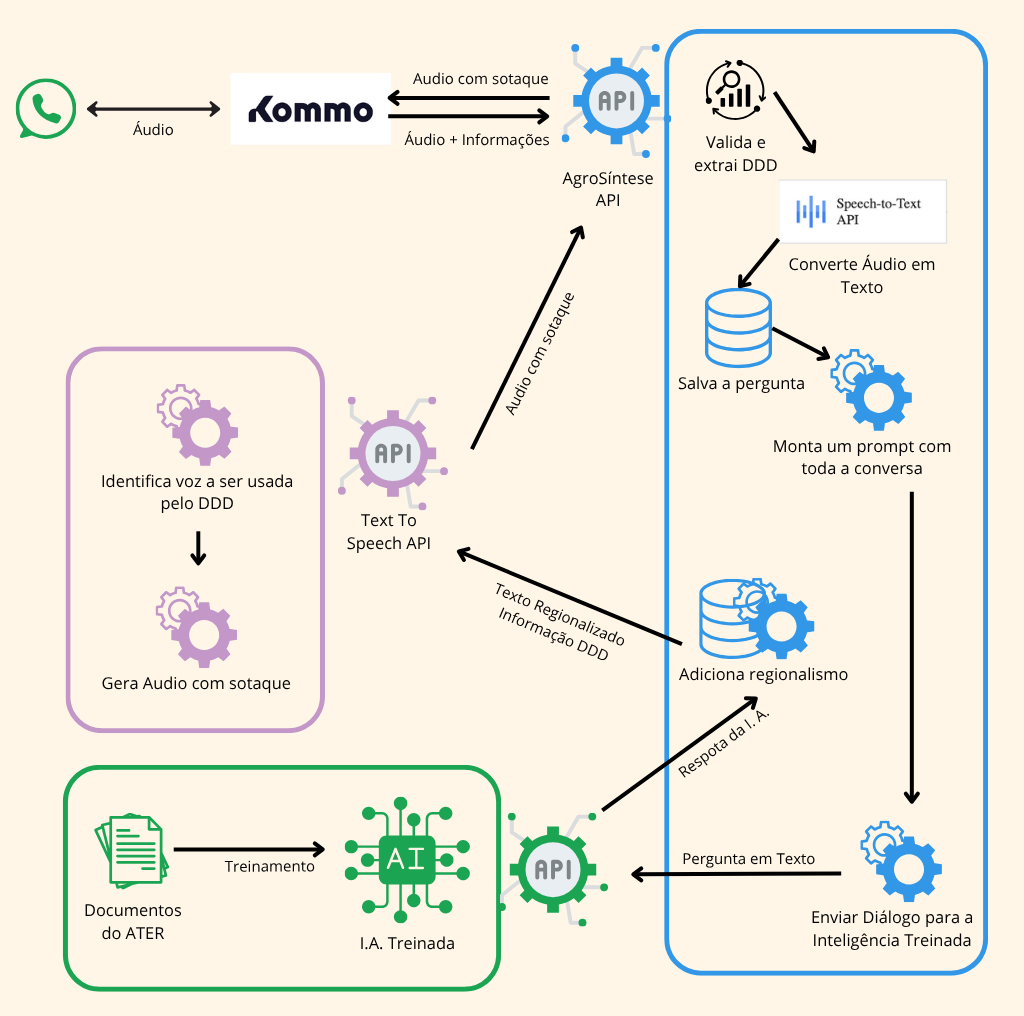
\includegraphics[width=1.0\linewidth,scale=1.0]{images/agro-sintese-arquitetura-03.png}
	\label{fig:whatsappfluxo}
\end{figure}


\section{Dicionários Regionais e Personalização Linguística}

A partir do mapeamento linguístico descrito na metodologia, serão criadas os registros contendo as expressões típicas, traduções técnicas e modos de tratamento apropriados para cada região do Brasil. Cada entrada recebe uma chave, definição técnica e equivalência popular, permitindo que a IA compreenda e produza linguagem próxima à realidade do usuário.

\section{Síntese de Voz e Empatia Digital}

Será utilizado o Coqui TTS para transformar as respostas textuais em voz com sotaques regionais. Serão gravadas amostras reais de falas de agricultores de diferentes regiões para o treinamento das vozes sintéticas. Esse componente terá papel fundamental na humanização do atendimento, promovendo acolhimento e empatia na comunicação com o agricultor.

\section{Interface e Telas do Sistema}

O sistema possuirá um painel administrativo com uma interface que será desenvolvida em Symfony, voltada aos técnicos responsáveis pelo acompanhamento das interações, atualização da base de dados e análise de indicadores de uso. 

As demais pessoas poderão interagir com o sistema diretamente pelo aplicativo do WhatsApp.
A ~\ref{fig:whatsapptela} mostra como a conversa fluirá, sendo que quando a conversa for iniciada com texto, o sistema develve um texto. Quando for iniciada por vóz, o sistema devolverá uma audio.

\begin{figure}[h]
	\centering
	\caption{Tela do WhatsApp conversando com o AgroSíntese }
	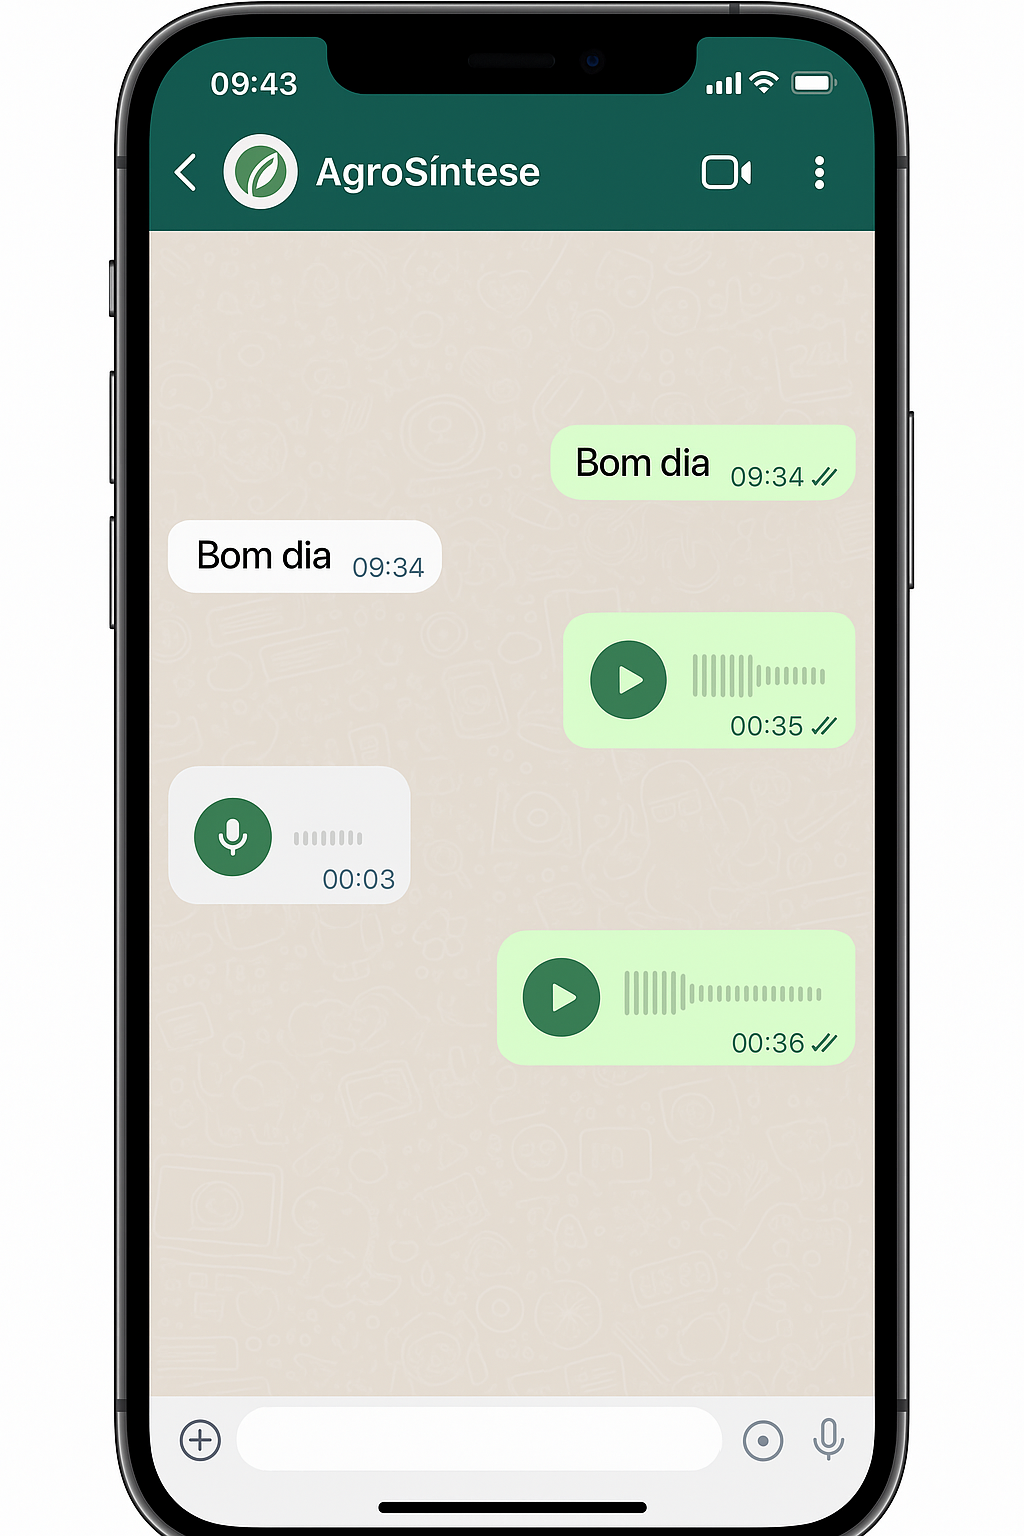
\includegraphics[width=0.5\linewidth,scale=1.0]{images/agro-sintese-whats.png}
	\label{fig:whatsapptela}
\end{figure}


As telas serão testadas com técnicos da extensão rural para garantir usabilidade, clareza e adaptabilidade em contextos de conectividade limitada.

\section{Funcionalidades do Painel Administrativo}

A plataforma AgroSíntese contará com um painel administrativo desenvolvido em Symfony, destinado a gestores e pesquisadores. Esse painel tem como objetivo permitir a manutenção do sistema, a gestão dos dados linguísticos e o acompanhamento das interações com os usuários.

O administrador poderá cadastrar, editar e excluir os sotaques de cada região, vinculando-os ao DDD correspondente. Além disso, é possível atualizar os dicionários regionais com novas expressões idiomáticas, termos populares e vocabulários técnicos específicos, garantindo a evolução contínua da base de conhecimento linguístico do sistema.

Outra funcionalidade importante do painel é o acesso completo ao histórico de conversas realizadas entre os agricultores e o sistema. O administrador pode visualizar todas as mensagens recebidas e enviadas, realizar buscas por palavras-chave, filtrar por DDD, data ou tema, e exportar os dados para análises posteriores. Essas informações são valiosas para fins de pesquisa, avaliação da efetividade comunicacional da plataforma e identificação de demandas recorrentes.

Essa camada administrativa torna o AgroSíntese uma ferramenta flexível e adaptável, permitindo sua atualização constante e o uso dos dados gerados como fonte para estudos acadêmicos, avaliação de políticas públicas e planejamento de ações de extensão rural mais eficazes.

\section{1.4.5 Interface e Telas do Sistema}

O painel administrativo do sistema AgroSíntese será projetado para facilitar a gestão de dados linguísticos e interações com agricultores de diversas regiões do Brasil. Com uma interface intuitiva, baseada no tema AdminKit, cada funcionalidade será adaptada para atender às necessidades do projeto. A seguir, estão descritas as principais telas a serem implementadas no sistema.

\subsubsection*{Tela de Listagem de Conversas}

\begin{figure}[H]
	\centering
	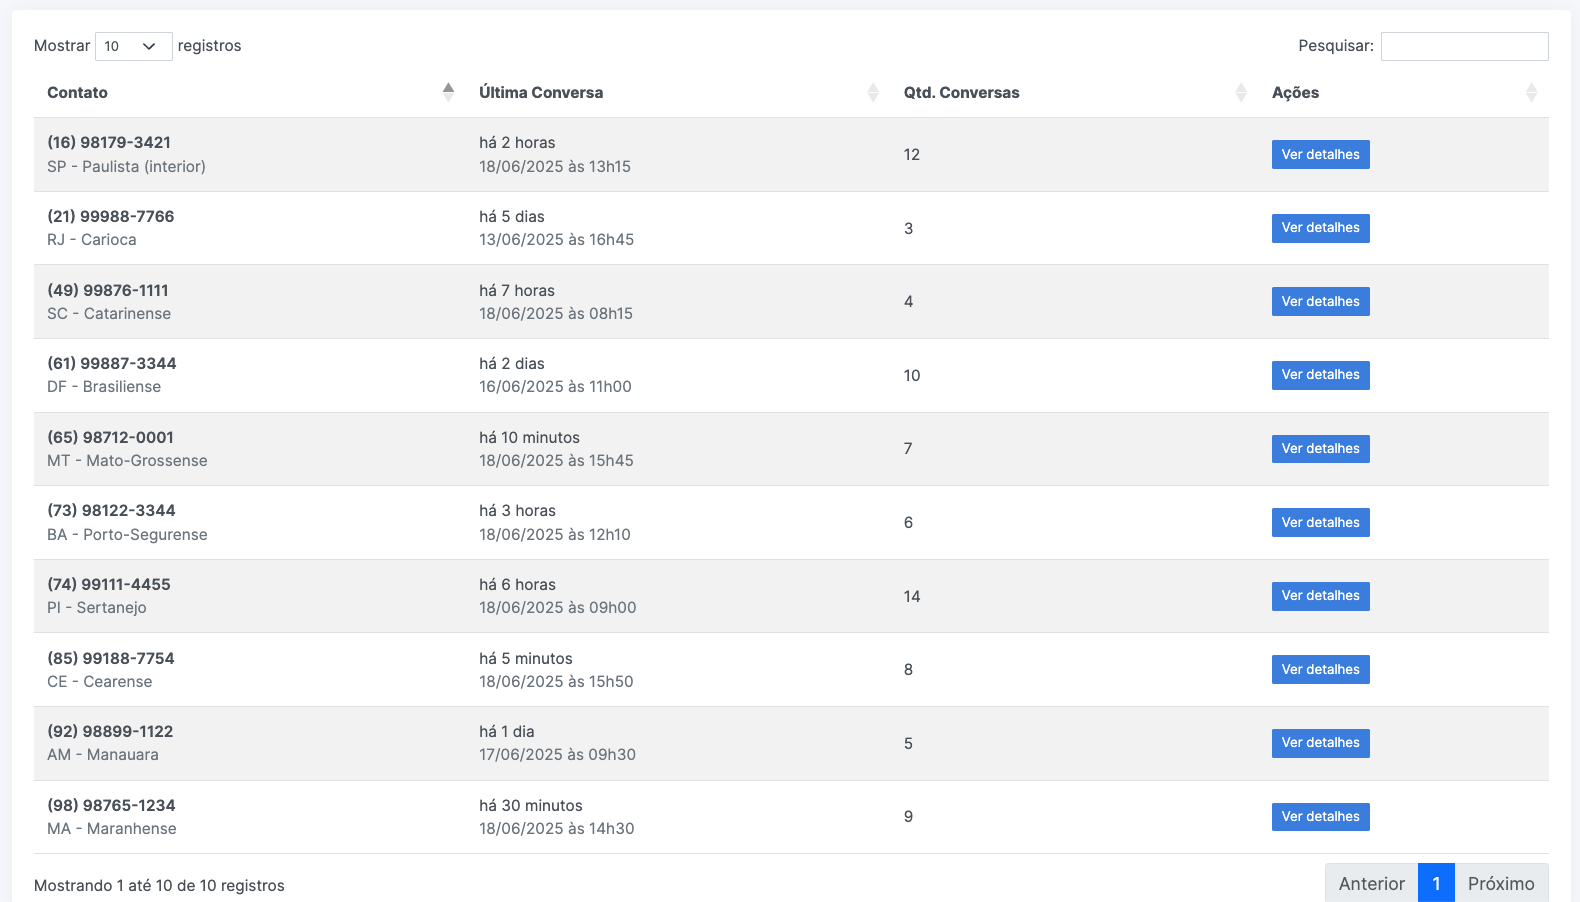
\includegraphics[width=0.95\linewidth]{images/adm-conversa-lista.png}
	\caption{Tela de listagem de conversas com agricultores. Exibe o número do telefone, dialeto associado, data da última conversa, e quantidade total de mensagens trocadas.}
\end{figure}

Essa tela é essencial para o acompanhamento das interações realizadas com os usuários do sistema. O administrador pode rapidamente verificar quais foram os últimos contatos, filtrando possíveis dúvidas recorrentes.

\subsubsection*{Tela de Detalhe da Conversa}

\begin{figure}[H]
	\centering
	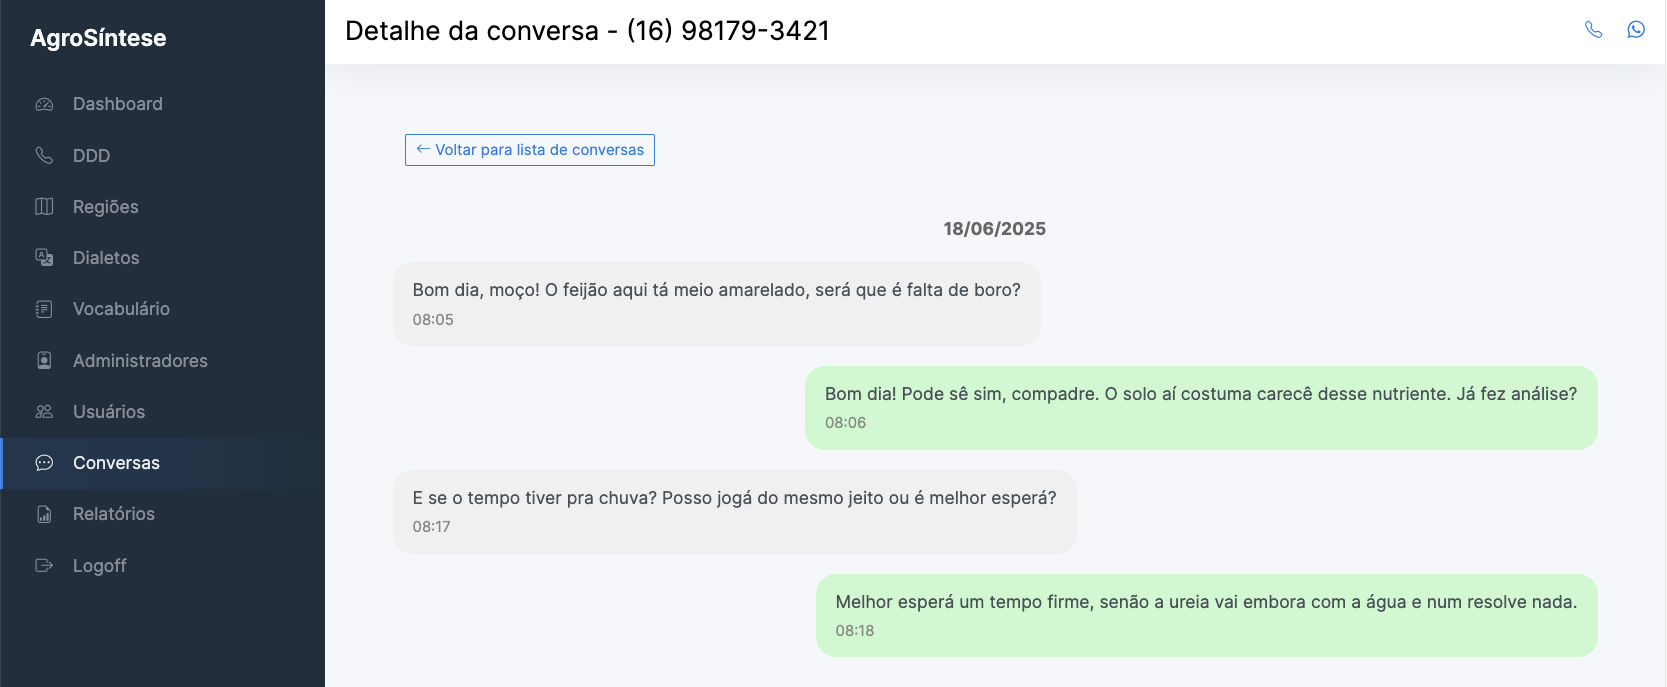
\includegraphics[width=0.95\linewidth]{images/adm-conversa-detalhe.png}
	\caption{Tela com detalhamento da conversa. As mensagens são exibidas em balões, com separação visual entre as falas do agricultor e as respostas da IA do sistema.}
\end{figure}

Este módulo simula um aplicativo de mensagens e permite visualizar a conversa de forma cronológica. A linguagem usada respeita os regionalismos, aproximando o tom da comunicação real dos agricultores.

\subsubsection*{Tela de Listagem de Dialetos Brasileiros}

\begin{figure}[H]
	\centering
	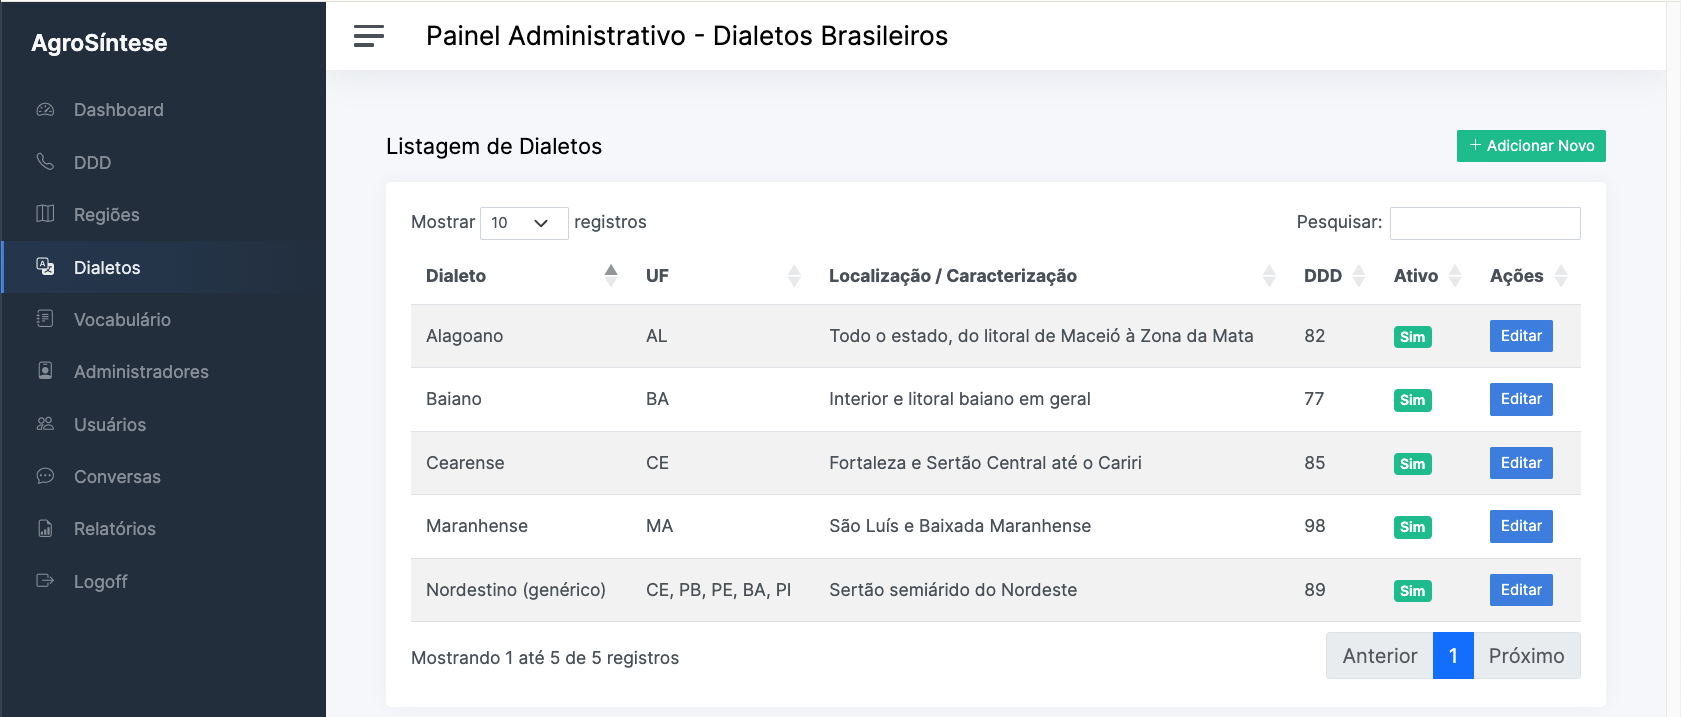
\includegraphics[width=0.95\linewidth]{images/adm-dialetos-braileito-lista.png}
	\caption{Tela de listagem de dialetos. Permite visualizar todos os dialetos cadastrados, com DDD, estado, nome, descrição e status.}
\end{figure}

Essa tela é usada para gerenciamento dos dialetos mapeados. Ela auxilia a associar corretamente as variantes regionais com os respectivos códigos DDD.

\subsubsection*{Formulário de Cadastro de Dialeto}

\begin{figure}[H]
	\centering
	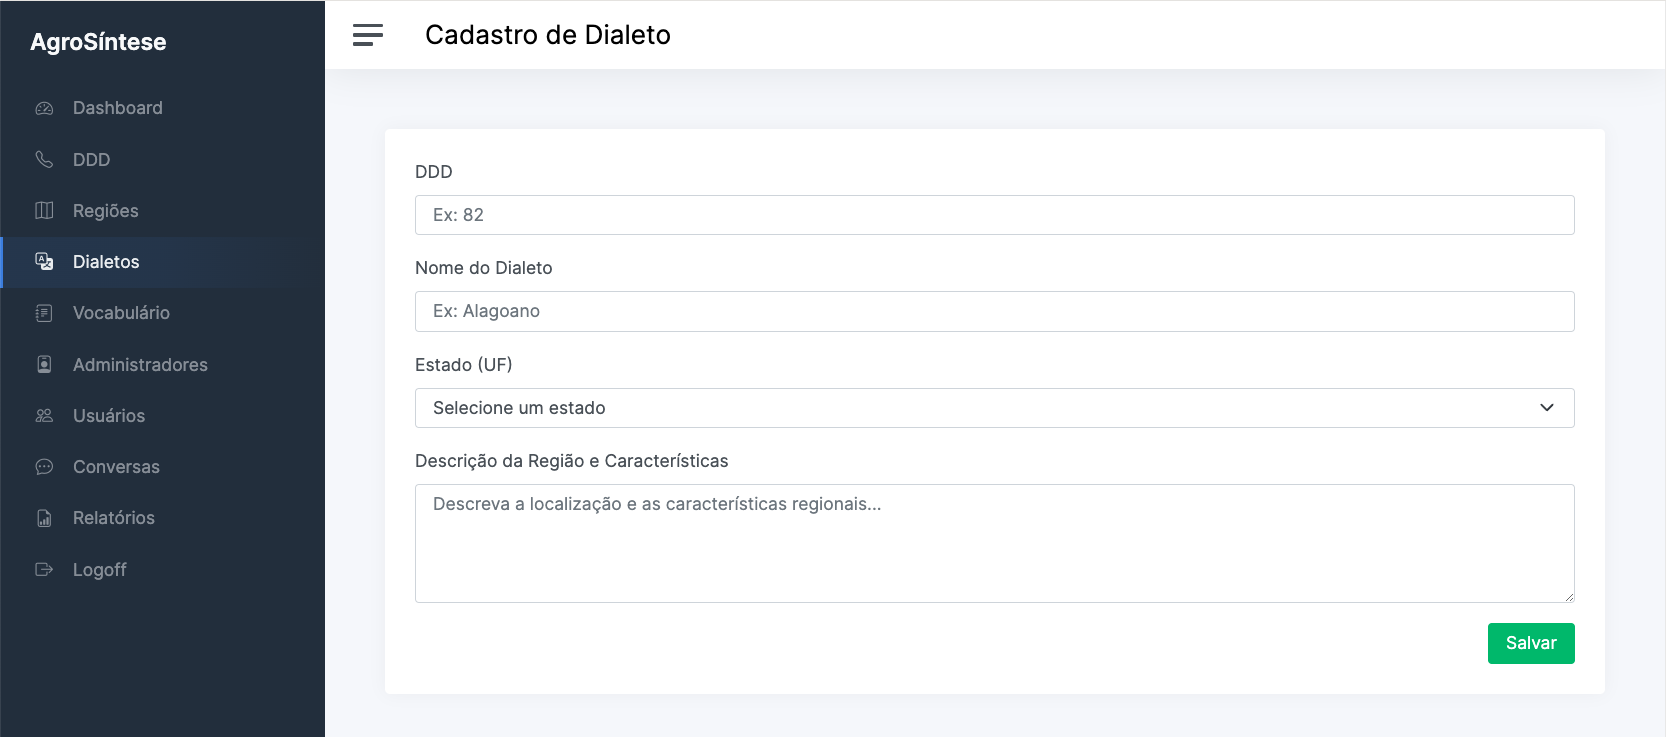
\includegraphics[width=0.95\linewidth]{images/adm-dialeto-form.png}
	\caption{Formulário utilizado para adicionar ou editar dialetos. Contém campos para DDD, estado, nome do dialeto e descrição das características regionais.}
\end{figure}

Permite a atualização ou inserção de novos dialetos no sistema. É possível incluir dialetos específicos de municípios, regiões ou estados, com total flexibilidade.

\subsubsection*{Tela de Listagem de Vocabulário Regional}

\begin{figure}[H]
	\centering
	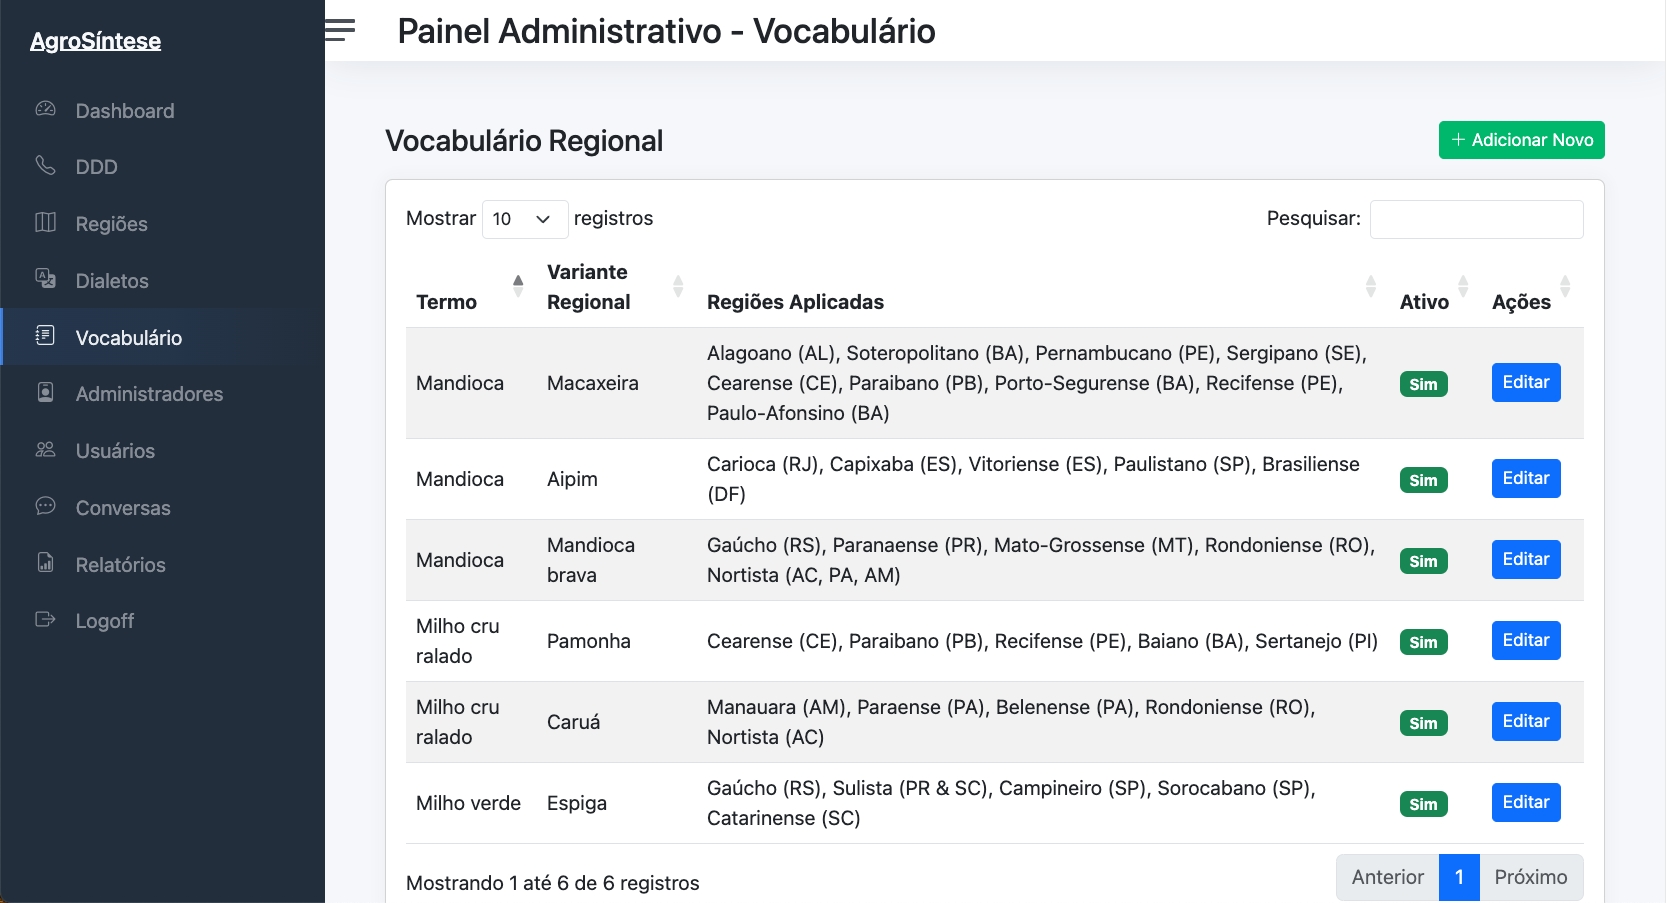
\includegraphics[width=0.95\linewidth]{images/adm-vocabulario-lista.png}
	\caption{Listagem de termos do vocabulário regional. Cada termo está associado a uma ou mais variantes e seus respectivos dialetos.}
\end{figure}

Esta tela organiza os termos populares usados em cada região. É essencial para que a IA do sistema compreenda e responda adequadamente às expressões utilizadas pelos usuários.

\subsubsection*{Formulário de Cadastro de Vocabulário}

\begin{figure}[H]
	\centering
	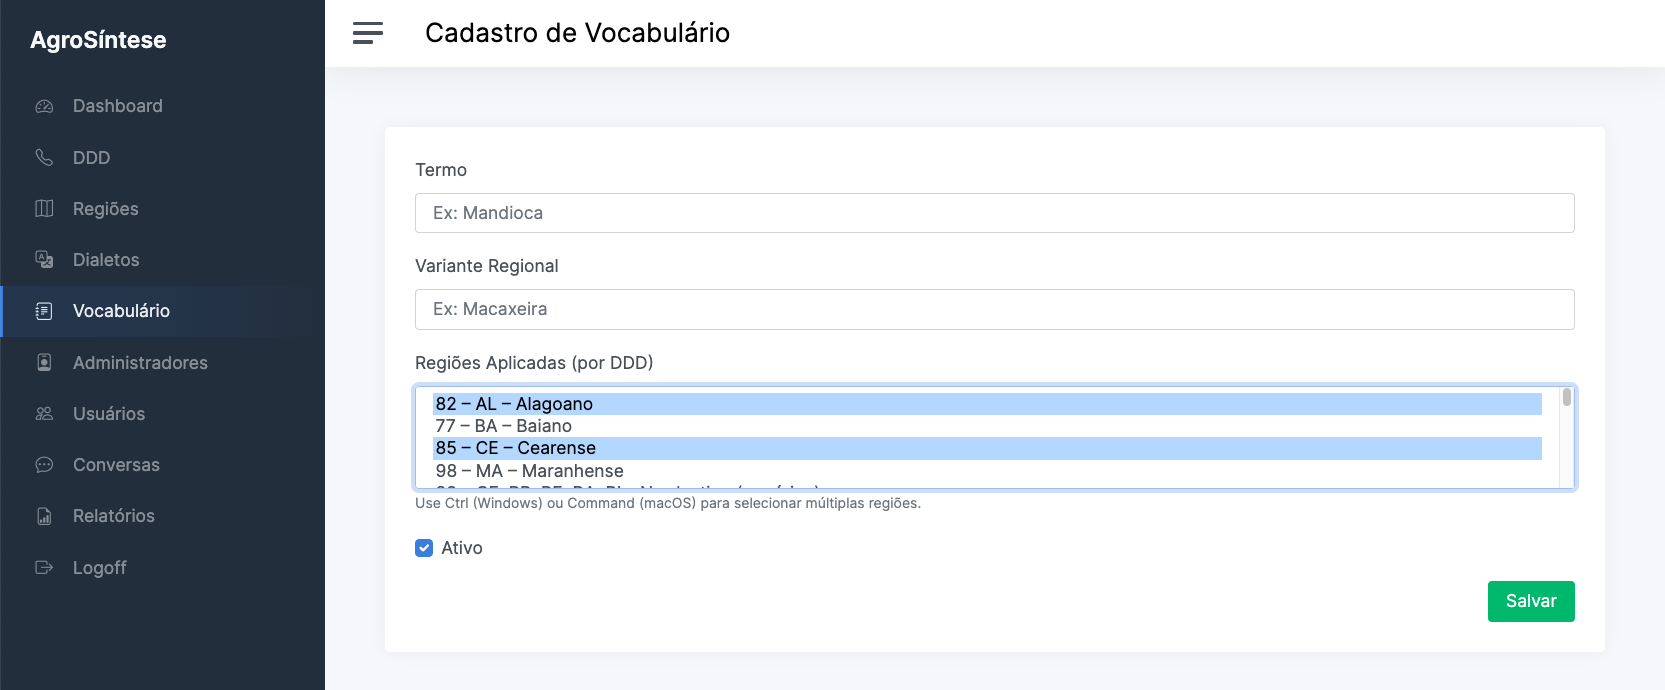
\includegraphics[width=0.95\linewidth]{images/adm-vocabulario-form.png}
	\caption{Formulário de vocabulário. Permite adicionar novos termos e associá-los a variantes e regiões específicas.}
\end{figure}

Através deste formulário, o administrador pode inserir termos usados localmente, como sinônimos populares para produtos agrícolas, ferramentas, condições climáticas, entre outros.

Cada uma dessas telas colabora diretamente para a missão do AgroSíntese: oferecer um atendimento técnico automatizado, dialógico e respeitoso com a diversidade linguística rural brasileira.


\section{Desafios Técnicos e Soluções Adotadas}

Alguns desafios enfrentados incluíram a oscilação da rede em zonas rurais, a limitação do WhatsApp para envio de áudios longos e a variação acentuada de vocabulário entre localidades vizinhas. Como solução, implementou-se um sistema de fallback textual e um banco de respostas pré-carregadas para consultas frequentes, acelerando o tempo de resposta em conexões instáveis.

---

O desenvolvimento do AgroSíntese, portanto, envolverá mais do que a construção de um software: constituiu-se como um processo de mediação sociotécnica, onde a linguagem, o território e o diálogo serão elementos estruturantes da arquitetura computacional. A seguir, são discutidos os resultados obtidos a partir da aplicação experimental da plataforma em campo.


\chapter*{Conclusão}

O desenvolvimento do sistema AgroSíntese representa um esforço significativo na direção da valorização dos saberes regionais e da construção de uma plataforma de assistência técnica rural automatizada, dialógica e situada. Fundamentado em autores como Bakhtin, Freire, Larrosa e Zuin, o projeto defende que o uso de tecnologias da informação deve respeitar a linguagem, a cultura e os contextos locais dos sujeitos do campo, evitando modelos centralizados e homogêneos de atendimento.

A estrutura técnica proposta, aliada à preocupação com os dialetos regionais e com as variantes vocabulares, cria as condições para que a futura inteligência artificial do sistema possa compreender e interagir com agricultores de diferentes partes do Brasil de maneira mais humana, acessível e eficaz. A interface administrativa desenvolvida permite cadastrar e organizar dialetos, vocabulários e conversas, estabelecendo as bases para o treinamento posterior da IA.

Embora o sistema ainda esteja em fase de prototipagem, os avanços realizados demonstram a viabilidade do projeto e sua aderência aos princípios da extensão rural crítica. A principal contribuição deste trabalho está na articulação entre fundamentos teóricos da comunicação e soluções técnicas baseadas em software livre e inteligência artificial.

\subsection*{Próximos Passos}

Para a continuidade e aprimoramento do AgroSíntese, os seguintes passos estão previstos:

\begin{itemize}
	\item Realizar entrevistas com agricultores e extensionistas de diferentes regiões do país, a fim de validar os dialetos e vocabulários levantados;
	\item Coletar e sistematizar materiais técnicos oriundos das políticas públicas de ATER (Assistência Técnica e Extensão Rural), como manuais, cartilhas, vídeos e podcasts;
	\item Treinar modelos de linguagem a partir das bases dialetais e vocabulários regionais reunidos;
	\item Avaliar o sistema com grupos focais e implementar melhorias com base no feedback recebido;
	\item Estudar a integração com canais reais de comunicação (como WhatsApp Business API), mantendo o foco na segurança, privacidade e acessibilidade dos usuários.
\end{itemize}

A consolidação do AgroSíntese como ferramenta de escuta e orientação técnica mediada por IA poderá ampliar o alcance das políticas públicas, fortalecer a autonomia dos agricultores e promover o reconhecimento das múltiplas vozes que constroem o campo brasileiro.
